% *********************************************************************
% © 2010–2026 Jeremy Sylvestre
%
% Permission is granted to copy, distribute and/or modify this document
% under the terms of the GNU Free Documentation License, Version 1.3 or
% any later version published by the Free Software Foundation; with no
% Invariant Sections, no Front-Cover Texts, and no Back-Cover Texts. A
% copy of the license is included in the appendix entitled “GNU Free
% Documentation License” that appears in the output document of this
% PreTeXt source code. All trademarks™ are the registered® marks of
% their respective owners.
%
% *********************************************************************

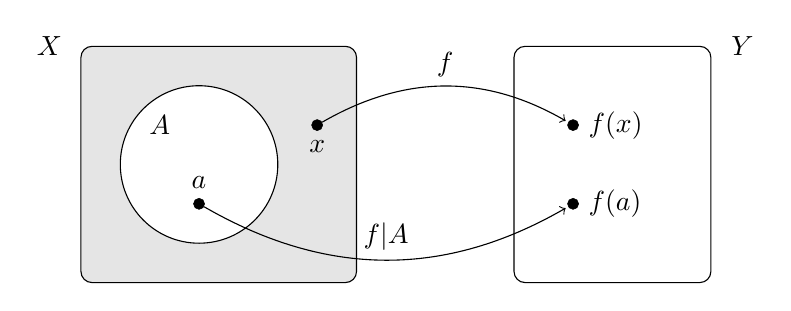
\begin{tikzpicture}[
	vertex/.style={ circle, draw, very thin, fill, inner sep=0pt, minimum size=4pt },
	vertexg/.style={ black!40!white, circle, draw, very thin, fill, inner sep=0pt, minimum size=4pt },
	vertexo/.style={ circle, draw, very thin, inner sep=0pt, minimum size=4pt }
]


\draw[rounded corners,fill=black!10!white] (-5,-1.5) rectangle (-1.5,1.5);
\node at (-5.4,1.5) {$X$};
\draw[fill=white] (-3.5,0) circle (1cm);
\node at (-4,0.5) {$A$};
\node at (-3.5,-0.5) (a) [vertex,label=above:{$a$}] {};
\node at (-2,0.5) (x) [vertex,label=below:{$x$}] {};
\draw[rounded corners] (0.5,-1.5) rectangle (3,1.5);
\node at (3.4,1.5) {$Y$};
\node at (1.25,-0.5) (b) [vertex,label=right:{$f(a)$}] {};
\draw[->,shorten >=1pt] (a) to [out=-30,in=-150] node[above] {$f|A$} (b);
\node at (1.25,0.5) (y) [vertex,label=right:{$f(x)$}] {};
\draw[->,shorten >=1pt] (x) to [out=30,in=150] node[above] {$f$} (y);

\end{tikzpicture}
